% ---------------------------------------------------------------------
% 2.7 Inteligencia artificial y aprendizaje automático
% ---------------------------------------------------------------------
\section[APRENDIZAJE AUTOMÁTICO]{Aprendizaje automático}

El aprendizaje automático es una rama de la inteligencia artificial que reúne métodos para
construir modelos a partir de los datos mediante el descubrimiento de patrones, para después
aplicarlos a datos nuevos de la misma naturaleza \cite{bishop2006}. Cuando los datos de
entrenamiento tienen etiquetas conocidas, el aprendizaje es supervisado, y es el caso de la
detección de la P300, que corresponde a un problema de clasificación binaria en el que cada época
está etiquetada como objetivo o no objetivo. El aprendizaje profundo, a su vez, es el subconjunto
del aprendizaje automático basado en redes neuronales con múltiples capas \cite{goodfellow2016}.

\subsection{Sobreajuste y generalización}

El objetivo de un modelo de aprendizaje automático no es reproducir los datos con los que fue
entrenado sino desempeñarse correctamente con datos que nunca ha visto, capacidad conocida como
generalización \cite{goodfellow2016}. Cuando un modelo es demasiado complejo para la cantidad de
datos disponibles, o se entrena durante demasiadas iteraciones, empieza a memorizar el ruido del
conjunto de entrenamiento. En ese momento, el error de entrenamiento sigue bajando, pero el error de
validación deja de disminuir y comienza a subir. Este fenómeno se conoce como sobreajuste y se
ilustra en la Figura~\ref{fig:sobreajuste} \cite{goodfellow2016,bishop2006}.
En el caso del EEG este riesgo es particularmente alto, pues las bases de datos suelen contener
pocos sujetos y un número limitado de épocas objetivo.

\begin{figure}[htbp]
\centering
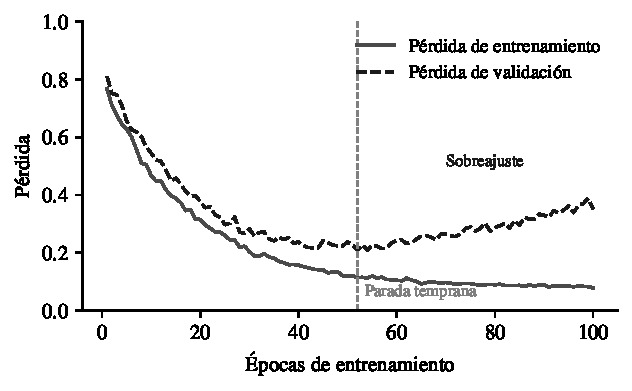
\includegraphics[width=0.68\textwidth]{02-marco-referencial/sobreajuste.pdf}
\caption{Curvas de pérdida de entrenamiento y validación: a partir de cierto punto el modelo
comienza a sobreajustarse. Elaboración propia.}
\label{fig:sobreajuste}
\end{figure}

\subsection{Esquemas de validación}

Para estimar la capacidad de generalización, los datos se dividen en tres conjuntos
\cite{goodfellow2016}. El de entrenamiento sirve para ajustar el modelo. El de validación se usa
para ajustar hiperparámetros y decidir cuándo detener el entrenamiento. El de prueba solo se
utiliza al final. La
validación cruzada de $k$ particiones repite este proceso $k$ veces rotando el subconjunto de
validación, lo que ofrece una estimación más estable cuando hay pocos datos \cite{bishop2006}. En
las BCI, además, se distinguen dos tipos de evaluación. En la evaluación intrasujeto, el modelo se
entrena y se prueba con datos de la misma persona. En la evaluación intersujeto, se prueba con una
persona que no participó en el entrenamiento \cite{alvarado2021}.
